\documentclass[a4paper,10pt,twoside]{article}
%\usepackage{amssymb}
%\usepackage{amsthm}
\usepackage[polish]{babel}
\usepackage[utf8]{inputenc}
\usepackage[T1]{fontenc}
\usepackage{indentfirst}
\usepackage{caption}
\usepackage[top=2.5cm, bottom=2.5cm, left=2.5cm, right=2.5cm]{geometry}
\usepackage{graphicx}
\usepackage{makecell}
\usepackage{amsmath}
\usepackage{booktabs}
\usepackage{multirow}
\usepackage{float}


\begin{document}
	
	\begin{center}
		\bgroup
		\def\arraystretch{1.5}
		\begin{tabular}{|c|c|c|c|c|c|}
			\hline
			EAIiIB & \multicolumn{2}{|c|}{Michał Kilian} & Rok II & \multicolumn{2}{|c|}{Grupa 5a} \\
			\hline
			\multicolumn{3}{|c|}{\begin{tabular}{c}Temat: \\ Wahadło proste \end{tabular}} & 
			\multicolumn{3}{|c|}{\begin{tabular}{c}Numer ćwiczenia: \\ 0 \end{tabular}} \\
			\hline
			\begin{tabular}{@{}c@{}}Data wykonania\\10.10.2018r.\end{tabular} & \begin{tabular}{@{}c@{}}Data oddania\\12.10.2018r.\end{tabular} & 
			\begin{tabular}{c}Zwrot do\\poprawki\\\phantom{data} \end{tabular} & \begin{tabular}{c}Data oddania\\\phantom{data}\end{tabular} &
			\begin{tabular}{@{}c@{}}Data zaliczenia\\\phantom{data}\end{tabular} & \begin{tabular}{c}Ocena\\\phantom{ocena}\end{tabular} \\[4ex]
			\hline
		\end{tabular}
		\egroup
	\end{center}

	\newpage
	\section{Cel ćwiczenia}
	Zaznajomienie się
	z typowymi metodami opracowania danych pomiarowych
	przy wykorzystaniu wyników pomiarów dla wahadła pro
	stego 
	

	Wahadło matematyczne to punktowa masa $m$ zawieszona na nieważkiej i nierozciągliwej lince poruszająca w jednorodnym polu grawitacyjnym.
	W doświadczeniu wykorzystamy bardzo dobre przybliżenie takiego układu jakim jest ciężka metalowa kulka zawieszona na nitce.
	
	Aby znacząco uprościć obliczenia przyjmiemy $\sin\theta\approx\theta$ co jest prawdą dla małych wartości kąta $\theta$ zgodnie z
	twierdzeniem Taylora. Dzięki temu ograniczamy wpływ oporu powietza na wyniki, a z uproszczonego równania ruchu wahadła
	uzyskujemy następujacą zależność
	\begin{equation}
	T=2\pi\sqrt{\frac{l}{g}}
	\end{equation}
	gdzie $T$ - okres drgań, $l$ - długość nici, $g$ - przyspieszenie grawitacyjne. Po przekształceniu otrzymujemy wzór roboczy pozwalający
	na wyznaczenie wartości przyspieszenia grawitacyjnego dla Ziemi
	\begin{equation}
	\label{eq:working_g}
	g=\frac{4\pi^2l}{T^2}
	\end{equation}
	\newpage
	\section{Wykonanie ćwiczenia}
	
	\begin{enumerate}
		\item Zapoznać się z budową mikroskopu
		\item Na obu powierzchniach płytki zrobić kreski, jedna nad drugą cienkim pisakiem (ewentualnie wykorzystać istniejące kreski)
		\item Zmierzyć śrubą
		mikrometryczną
		grubość płytki d w pobliżu kresek. 
		\item Ustaw  badaną
		płytkę
		na  stoliku  mikroskopu  w  uchwycie  i  dobierz  ostrość
		tak  by  uzyskać
		kontrastowy obraz. Regulując położenie stolika pokrętłem 7a zaobserwuj górny i dolny 
		ślad zaznaczony na płytce. 
		\item Pokrętłem 7b przesuń stolik mikroskopu do momentu uzyskania ostrego obrazu śladu na górnej powierzchni płytki.
		\item Odczytaj położenie $a_g$ wskazówki czujnika mikrometrycznego. 
		\item Przesuń stolik mikroskopu do położenia, w którym widoczny jest ślad na dolnej powierzchni płytki (pokrętłem 7b). 
		\item Ponownie odczytaj położenie $a_d$ wskazówki czujnika.
		\item Odczyty zanotuj w tabeli 1, 2 lub 3.
	\end{enumerate}

	
	\section{Wyniki pomiarów}
	
\begin{table}[htb]
	\begin{tabular}{|c|c|c|c|c|c|}
		\hline
		Indeks & Lp {[}H{]} & Lz {[}H{]} & odległość[cm] & Indukcyjność wzajemna {[}H{]} & Współczynnik sprzężenia k \\ \hline
		1      & 2,69       & 3,67 & 0       & 0,25                          & 0,43                      \\ \hline
		2      & 2,69       & 3,65 & 0,5     & 0,24                          & 0,42                      \\ \hline
		3      & 2,7        & 3,63 & 1       & 0,23                          & 0,40                      \\ \hline
		4      & 2,71       & 3,61 & 1,5     & 0,23                          & 0,39                      \\ \hline
		5      & 2,72       & 3,59 & 2       & 0,22                          & 0,38                      \\ \hline
		6      & 2,74       & 3,58 & 2,5     & 0,21                          & 0,37                      \\ \hline
		7      & 2,76       & 3,55 & 3       & 0,20                          & 0,34                      \\ \hline
		8      & 2,78       & 3,53 & 3,5     & 0,19                          & 0,33                      \\ \hline
		9      & 2,81       & 3,5  & 4       & 0,17                          & 0,30                      \\ \hline
		10     & 2,83       & 3,46 & 4,5     & 0,16                          & 0,27                      \\ \hline
		11     & 2,86       & 3,43 & 5       & 0,14                          & 0,25                      \\ \hline
		12     & 2,88       & 3,41 & 5,5     & 0,13                          & 0,23                      \\ \hline
		13     & 2,91       & 3,37 & 6       & 0,12                          & 0,20                      \\ \hline
		14     & 2,94       & 3,35 & 6,5     & 0,10                          & 0,18                      \\ \hline
		15     & 2,96       & 3,32 & 7       & 0,09                          & 0,16                      \\ \hline
		16     & 2,99       & 3,29 & 7,5     & 0,08                          & 0,13                      \\ \hline
		17     & 3,01       & 3,27 & 8       & 0,07                          & 0,11                      \\ \hline
		18     & 3,03       & 3,25 & 8,5     & 0,06                          & 0,10                      \\ \hline
		19     & 3,05       & 3,23 & 9       & 0,05                          & 0,08                      \\ \hline
		20     & 3,06       & 3,22 & 9,5     & 0,04                          & 0,07                      \\ \hline
		21     & 3,08       & 3,21 & 10      & 0,03                          & 0,06                      \\ \hline
		22     & 3,09       & 3,19 & 10,5    & 0,03                          & 0,04                      \\ \hline
		23     & 3,11       & 3,18 & 11      & 0,02                          & 0,03                      \\ \hline
		24     & 3,11       & 3,17 & 11,5    & 0,02                          & 0,03                      \\ \hline
		25     & 3,11       & 3,17 & 12      & 0,02                          & 0,03                      \\ \hline
		26     & 3,12       & 3,16 & 12,5    & 0,01                          & 0,02                      \\ \hline
		27     & 3,12       & 3,16 & 13      & 0,01                          & 0,02                      \\ \hline
		28     & 3,12       & 3,16 & 13,5    & 0,01                          & 0,02                      \\ \hline
		29     & 3,12       & 3,16 & 14      & 0,01                          & 0,02                      \\ \hline
		30     & 3,12       & 3,16 & 14,5    & 0,01                          & 0,02                      \\ \hline
	\end{tabular}
\end{table}
\noindent
Indukcyjność własna $L_1 = 3,00$\\
Indukcyjność własna $L_2 = 0,11$

 \newpage
	
	\section{Opracowanie wyników pomiarów}
	\begin{enumerate}
		\item \textit{Obliczyć
			współczynniki  indukcji  wzajemnej 
			M
			oraz  współczynnika  sprzężenia 
			k
			dla  każdego  położenia 
			cewek. }\vspace{10pt}
		\\ Współczynnik M indukcyjności wzajemnej liczony był ze wzoru 
		$$ M = \frac{L_z - L_p}{4}$$ natomiast współczynnik k ze wzoru 
		$$k = \frac{M}{\sqrt{L_1 L_2}} $$ Wyniki zostały zawarte w tabeli.
		\item \textit{ Dla  cewki  powietrznej  wykonać
		wykres  zależności  wypadkowej  indukcyjności  układu  (sprzężenie  dodatnie
		i ujemne) oraz współczynnika sprzężenia 
		k
		od odległości cewek}\vspace{10pt} \\Wykresy zostały zamieszczone poniżej
		\item \textit{Skomentować wyniki}
	\end{enumerate}
	\begin{figure}[H]
		\centering{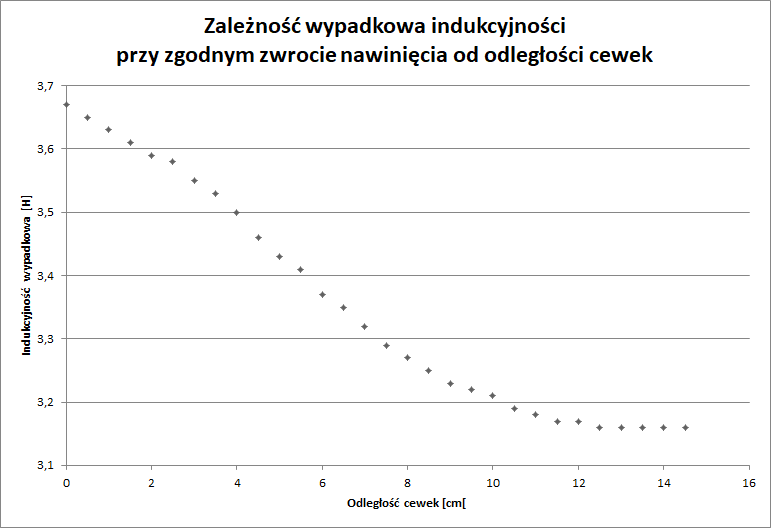
\includegraphics[scale=0.6]{W1}}
	\end{figure}
		\begin{figure}[H]
		\centering{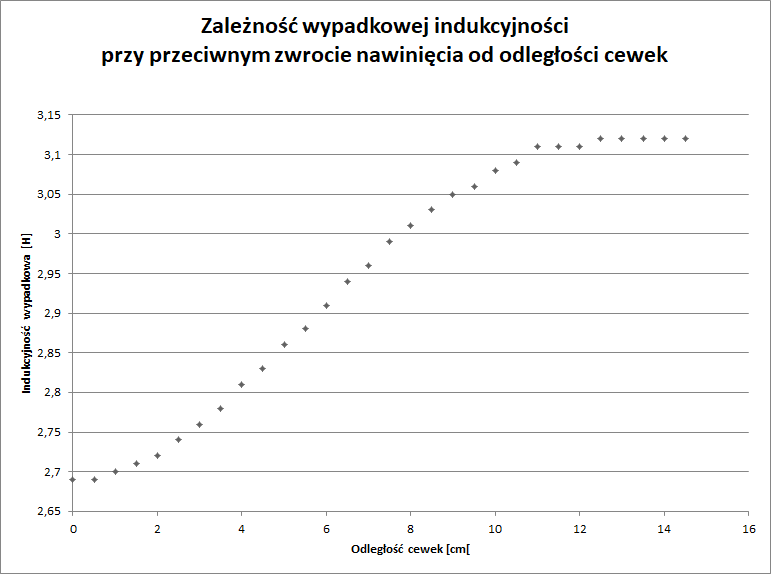
\includegraphics[scale=0.6]{W2}}
	\end{figure}
	\begin{figure}[H]
	\centering{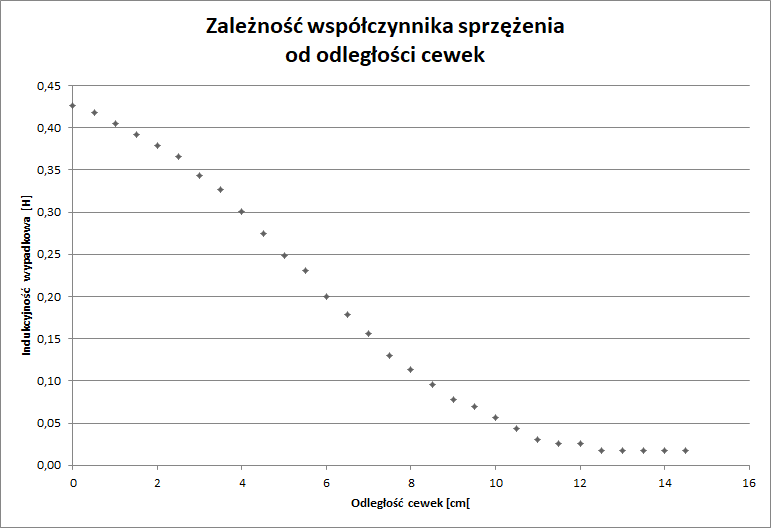
\includegraphics[scale=0.6]{W3}}
	\end{figure}
 \newpage

	\section{Wnioski}

\end{document}
















\end{}